\documentclass[11pt,article]{memoir}

\usepackage{amsmath,amssymb,amsthm}
\usepackage{mathrsfs}
\usepackage{geometry}
\usepackage{hyperref}
\usepackage{enumitem}
\usepackage{booktabs}
\usepackage{array}
\usepackage{tikz}
\usepackage{pgfplots}
\usepackage{algorithm}
\usepackage{algpseudocode}
\usepackage{listings}
\usepackage{xcolor}
\usepackage{graphicx}
\usepackage{caption}
\usepackage{subcaption}
\usepackage{pifont}
\usepackage{graphicx}

\geometry{margin=1in}
\pgfplotsset{compat=1.18}

% Code listing style
\lstset{
    language=Python,
    basicstyle=\ttfamily\small,
    keywordstyle=\color{blue},
    commentstyle=\color{green!60!black},
    stringstyle=\color{red!70!black},
    numbers=left,
    numberstyle=\tiny\color{gray},
    numbersep=5pt,
    frame=single,
    breaklines=true,
    captionpos=b
}

% Theorem environments
\theoremstyle{plain}
\newtheorem{theorem}{Theorem}[section]
\newtheorem{proposition}[theorem]{Proposition}
\newtheorem{lemma}[theorem]{Lemma}
\newtheorem{corollary}[theorem]{Corollary}
\newtheorem{conjecture}[theorem]{Conjecture}

\theoremstyle{definition}
\newtheorem{definition}[theorem]{Definition}
\newtheorem{example}[theorem]{Example}
\newtheorem{remark}[theorem]{Remark}
\newtheorem{algorithm_def}[theorem]{Algorithm}

% Custom commands
\newcommand{\R}{\mathbb{R}}
\newcommand{\Z}{\mathbb{Z}}
\newcommand{\N}{\mathbb{N}}
\newcommand{\C}{\mathbb{C}}

\title{\textbf{Visualizing Prime Numbers Through the $E_8$ Lattice}\\[0.5em]
\large A Pedagogical Guide to the Mathematics Behind\\
$E_8$ Projection Slope Coloring of the Ulam Spiral}

\author{A Tutorial on Exceptional Geometry in Number Theory}
\date{\today}

\begin{document}

\maketitle

\begin{abstract}
This tutorial provides a complete, self-contained guide to creating visualizations that reveal hidden structure in the distribution of prime numbers using the exceptional Lie algebra $E_8$. We develop each mathematical component from first principles: the $E_8$ root lattice, prime gap normalization, root assignment algorithms, two-dimensional projection, and the Ulam spiral coordinate system. The resulting visualization---primes colored by their $E_8$ projection slope---reveals striking concentric ring patterns that demonstrate primes are not randomly distributed in $E_8$ root space but follow coherent wave-like structures. We provide complete algorithms and code, enabling readers to reproduce and extend these results.
\end{abstract}

\tableofcontents

\newpage

%==============================================================================
\chapter{Introduction}
%==============================================================================

\section{The Mystery of Prime Distribution}

Prime numbers---integers greater than 1 divisible only by 1 and themselves---have fascinated mathematicians for millennia. Despite their simple definition, their distribution among the integers exhibits both regularity and apparent randomness that has resisted complete understanding.

The \textbf{Prime Number Theorem} tells us that the number of primes up to $x$, denoted $\pi(x)$, satisfies:
\begin{equation}
\pi(x) \sim \frac{x}{\ln x} \quad \text{as } x \to \infty
\end{equation}

This gives the ``density'' of primes but says nothing about their precise locations. The gaps between consecutive primes, $g_n = p_{n+1} - p_n$, appear erratic when examined individually.

\section{The Ulam Spiral: A Visual Discovery}

In 1963, mathematician Stanislaw Ulam, while doodling during a boring meeting, arranged the positive integers in a square spiral and marked the primes. To his surprise, the primes clustered along diagonal lines:

\begin{center}
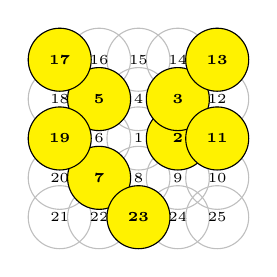
\begin{tikzpicture}[scale=0.5]
    % Draw the spiral numbers
    \foreach \n/\x/\y in {1/0/0, 2/1/0, 3/1/1, 4/0/1, 5/-1/1, 6/-1/0, 7/-1/-1, 8/0/-1, 9/1/-1, 10/2/-1, 11/2/0, 12/2/1, 13/2/2, 14/1/2, 15/0/2, 16/-1/2, 17/-2/2, 18/-2/1, 19/-2/0, 20/-2/-1, 21/-2/-2, 22/-1/-2, 23/0/-2, 24/1/-2, 25/2/-2} {
        \node[circle, minimum size=0.8cm, draw=gray!50, font=\tiny] at (\x, \y) {\n};
    }
    % Highlight primes
    \foreach \n/\x/\y in {2/1/0, 3/1/1, 5/-1/1, 7/-1/-1, 11/2/0, 13/2/2, 17/-2/2, 19/-2/0, 23/0/-2} {
        \node[circle, minimum size=0.8cm, fill=yellow, draw=black, font=\tiny\bfseries] at (\x, \y) {\n};
    }
\end{tikzpicture}
\end{center}

The diagonal clustering corresponds to prime-generating quadratic polynomials like Euler's famous $n^2 + n + 41$, which produces 40 consecutive primes for $n = 0, 1, \ldots, 39$.

\section{Our Goal: Revealing Deeper Structure with $E_8$}

This tutorial develops a visualization technique that goes beyond simply marking primes. We will:

\begin{enumerate}
    \item Encode each prime's \textbf{gap} (distance to the next prime) as a position in the 8-dimensional $E_8$ root lattice
    \item \textbf{Project} this 8D information down to a 2D ``slope'' value
    \item \textbf{Color} each prime in the Ulam spiral according to this slope
\end{enumerate}

The result reveals \textbf{concentric ring patterns} showing that the $E_8$ encoding of primes evolves coherently---not randomly---as we move outward through the spiral.

% Basic usage \includegraphics{example.png} % With scaling \includegraphics[scale=0.5]{example.png} % With width specification \includegraphics[width=0.8\textwidth]{example.png} 
% Inside a figure environment (for captions and labels) 

\begin{center}
	\begin{figure}[h] 
		\centering 
		\includegraphics[width=1\textwidth]{primes.png}
		\caption{$E_8$ encoding of primes} 
		\label{fig:example} 
	\end{figure}
\end{center}


\section{Prerequisites}

This tutorial assumes familiarity with:
\begin{itemize}
    \item Basic linear algebra (vectors, matrices, norms)
    \item Elementary number theory (primes, divisibility)
    \item Python programming (NumPy, Matplotlib)
\end{itemize}

We will develop all $E_8$-specific mathematics from scratch.

%==============================================================================
\chapter{The $E_8$ Root Lattice}
%==============================================================================

\section{What is $E_8$?}

$E_8$ is the largest of the five \textbf{exceptional simple Lie algebras}. While this abstract algebraic definition requires graduate-level mathematics, we can work directly with its concrete realization as a lattice in $\R^8$.

\begin{definition}[$E_8$ Lattice]
The $E_8$ lattice $\Lambda_{E_8} \subset \R^8$ consists of all points $(x_1, x_2, \ldots, x_8)$ satisfying:
\begin{enumerate}
    \item All coordinates are integers, OR all coordinates are half-integers (i.e., of the form $n + \frac{1}{2}$ for integer $n$)
    \item The sum of all coordinates is even: $\sum_{i=1}^8 x_i \equiv 0 \pmod{2}$
\end{enumerate}
\end{definition}

\begin{example}
The following are $E_8$ lattice points:
\begin{itemize}
    \item $(1, 1, 0, 0, 0, 0, 0, 0)$ --- integers summing to 2 (even) \checkmark
    \item $(\frac{1}{2}, \frac{1}{2}, \frac{1}{2}, \frac{1}{2}, \frac{1}{2}, \frac{1}{2}, \frac{1}{2}, \frac{1}{2})$ --- half-integers summing to 4 (even) \checkmark
    \item $(1, 0, 0, 0, 0, 0, 0, 0)$ --- integers summing to 1 (odd) \ding{55}
    \item $(\frac{1}{2}, \frac{1}{2}, \frac{1}{2}, 0, 0, 0, 0, 0)$ --- mixed integers/half-integers \ding{55}
\end{itemize}
\end{example}

\section{The 240 Root Vectors}

The \textbf{roots} of $E_8$ are the lattice points closest to the origin (excluding the origin itself). All roots have the same Euclidean norm.

\begin{proposition}
The $E_8$ root system $\Phi_{E_8}$ contains exactly 240 vectors, all of norm $\sqrt{2}$.
\end{proposition}

These 240 roots divide into two types:

\subsection{Type I Roots (112 vectors)}

These have two coordinates equal to $\pm 1$ and six coordinates equal to 0:
\begin{equation}
\text{Type I}: \quad (\ldots, \pm 1, \ldots, \pm 1, \ldots) \quad \text{with 6 zeros}
\end{equation}

\textbf{Counting}: Choose 2 positions from 8 for the non-zero entries ($\binom{8}{2} = 28$ ways), then choose signs ($2^2 = 4$ ways):
\begin{equation}
|\text{Type I}| = \binom{8}{2} \times 2^2 = 28 \times 4 = 112
\end{equation}

\begin{example}
Type I roots include:
\begin{align*}
&(1, 1, 0, 0, 0, 0, 0, 0), \quad (1, -1, 0, 0, 0, 0, 0, 0) \\
&(1, 0, 1, 0, 0, 0, 0, 0), \quad (0, 0, 0, 0, 0, 0, -1, -1)
\end{align*}
\end{example}

\subsection{Type II Roots (128 vectors)}

These have all coordinates equal to $\pm\frac{1}{2}$, with an \textbf{even number of minus signs}:
\begin{equation}
\text{Type II}: \quad \left(\pm\frac{1}{2}, \pm\frac{1}{2}, \pm\frac{1}{2}, \pm\frac{1}{2}, \pm\frac{1}{2}, \pm\frac{1}{2}, \pm\frac{1}{2}, \pm\frac{1}{2}\right) \quad \text{even \# of } -\frac{1}{2}\text{'s}
\end{equation}

\textbf{Counting}: Of the $2^8 = 256$ possible sign choices, exactly half have an even number of minus signs:
\begin{equation}
|\text{Type II}| = \frac{256}{2} = 128
\end{equation}

\begin{example}
Type II roots include:
\begin{align*}
&\left(\frac{1}{2}, \frac{1}{2}, \frac{1}{2}, \frac{1}{2}, \frac{1}{2}, \frac{1}{2}, \frac{1}{2}, \frac{1}{2}\right) \quad \text{(0 minus signs)} \\
&\left(-\frac{1}{2}, -\frac{1}{2}, \frac{1}{2}, \frac{1}{2}, \frac{1}{2}, \frac{1}{2}, \frac{1}{2}, \frac{1}{2}\right) \quad \text{(2 minus signs)} \\
&\left(-\frac{1}{2}, -\frac{1}{2}, -\frac{1}{2}, -\frac{1}{2}, \frac{1}{2}, \frac{1}{2}, \frac{1}{2}, \frac{1}{2}\right) \quad \text{(4 minus signs)}
\end{align*}
\end{example}

\textbf{Verification of norm}: For Type II,
\begin{equation}
\|v\|^2 = 8 \times \left(\frac{1}{2}\right)^2 = 8 \times \frac{1}{4} = 2 \quad \Rightarrow \quad \|v\| = \sqrt{2}
\end{equation}

\section{Generating the Roots in Code}

\begin{algorithm}
\caption{Generate all 240 $E_8$ root vectors}
\begin{algorithmic}[1]
\State $\text{roots} \gets []$
\Comment{Type I: 112 roots}
\For{$i = 0$ to $7$}
    \For{$j = i+1$ to $7$}
        \For{$s_1 \in \{-1, +1\}$}
            \For{$s_2 \in \{-1, +1\}$}
                \State $v \gets (0, 0, 0, 0, 0, 0, 0, 0)$
                \State $v[i] \gets s_1$; $v[j] \gets s_2$
                \State Append $v$ to roots
            \EndFor
        \EndFor
    \EndFor
\EndFor
\Comment{Type II: 128 roots}
\For{mask $= 0$ to $255$}
    \State $\text{signs} \gets$ [bit $i$ of mask $\to \pm 1$]
    \If{number of $-1$'s is even}
        \State $v \gets (\text{signs}[i] \times 0.5$ for $i = 0, \ldots, 7)$
        \State Append $v$ to roots
    \EndIf
\EndFor
\State \Return roots \Comment{240 vectors}
\end{algorithmic}
\end{algorithm}

\section{Why $E_8$?}

The $E_8$ lattice has remarkable properties:

\begin{enumerate}
    \item \textbf{Densest packing}: In 8 dimensions, $E_8$ achieves the densest possible sphere packing (proven by Viazovska, 2016).

    \item \textbf{Self-dual}: $\Lambda_{E_8}^* = \Lambda_{E_8}$ (the dual lattice equals itself).

    \item \textbf{Even}: All vectors have even squared norm ($\|v\|^2 \in 2\Z$).

    \item \textbf{Kissing number 240}: Each sphere in the packing touches exactly 240 others.
\end{enumerate}

The number 248 appears throughout: the Lie algebra $\mathfrak{e}_8$ has dimension 248, decomposing as $248 = 8 + 240$ (Cartan subalgebra plus root spaces).

For our purposes, $E_8$ provides a rich, rigid structure for encoding 1-dimensional information (prime gaps) in a way that preserves geometric relationships.

%==============================================================================
\chapter{Prime Gaps and Normalization}
%==============================================================================

\section{Prime Gaps}

\begin{definition}
The $n$-th \textbf{prime gap} is:
\begin{equation}
g_n = p_{n+1} - p_n
\end{equation}
where $p_n$ denotes the $n$-th prime number.
\end{definition}

\begin{example}
The first several prime gaps:
\begin{center}
\begin{tabular}{c|cccccccccc}
$n$ & 1 & 2 & 3 & 4 & 5 & 6 & 7 & 8 & 9 & 10 \\
\hline
$p_n$ & 2 & 3 & 5 & 7 & 11 & 13 & 17 & 19 & 23 & 29 \\
$g_n$ & 1 & 2 & 2 & 4 & 2 & 4 & 2 & 4 & 6 & 2
\end{tabular}
\end{center}
\end{example}

Prime gaps grow slowly on average but can be arbitrarily large. The famous \textbf{twin prime conjecture} asserts that $g_n = 2$ infinitely often.

\section{The Need for Normalization}

Raw gaps $g_n$ grow with the size of primes. The Prime Number Theorem implies:
\begin{equation}
\mathbb{E}[g_n] \approx \ln p_n
\end{equation}

To compare gaps across different magnitudes, we normalize:

\begin{definition}[Normalized Gap]
The \textbf{normalized prime gap} is:
\begin{equation}
\tilde{g}_n = \frac{g_n}{\ln p_n}
\end{equation}
\end{definition}

\begin{proposition}
The normalized gaps have mean approximately 1:
\begin{equation}
\lim_{N \to \infty} \frac{1}{N} \sum_{n=1}^{N} \tilde{g}_n = 1
\end{equation}
\end{proposition}

This follows from the Prime Number Theorem: if there are approximately $x/\ln x$ primes up to $x$, then the average gap near $x$ is approximately $\ln x$.

\section{Distribution of Normalized Gaps}

Normalized gaps cluster around 1 but have a wide distribution:

\begin{itemize}
    \item Small gaps ($\tilde{g}_n < 0.5$): Twin primes and close pairs
    \item Typical gaps ($0.5 < \tilde{g}_n < 2$): Most primes
    \item Large gaps ($\tilde{g}_n > 2$): Prime deserts
\end{itemize}

The variance of normalized gaps is approximately 1, and the distribution is roughly exponential for small values with a long tail.

\section{Implementation}

\begin{lstlisting}[caption={Computing normalized prime gaps}]
import numpy as np

def compute_normalized_gaps(primes):
    """
    Compute normalized gaps g_n / log(p_n)

    Args:
        primes: numpy array of prime numbers

    Returns:
        normalized_gaps: array of length len(primes) - 1
    """
    # Compute raw gaps
    gaps = np.diff(primes.astype(np.float64))

    # Compute log of each prime (except the last)
    log_primes = np.log(primes[:-1].astype(np.float64))

    # Avoid division by zero for p=2
    log_primes[log_primes < 1] = 1

    # Normalize
    normalized_gaps = gaps / log_primes

    return normalized_gaps
\end{lstlisting}

%==============================================================================
\chapter{The Root Assignment Algorithm}
%==============================================================================

\section{Mapping Gaps to $E_8$ Roots}

We now develop the key algorithm: assigning each normalized prime gap to one of the 240 $E_8$ root vectors.

\subsection{The Core Idea}

All 240 roots have the same norm $\sqrt{2} \approx 1.414$. We use the \textbf{normalized gap magnitude} to determine a ``phase'' that selects among the roots.

\begin{definition}[Root Assignment]
For a normalized gap $\tilde{g}$, define:
\begin{equation}
\phi(\tilde{g}) = \arg\min_{v \in \Phi_{E_8}} \left| \|v\| - \sqrt{\tilde{g}} \right|
\end{equation}
Since all roots have $\|v\| = \sqrt{2}$, this selects the root whose norm is closest to $\sqrt{\tilde{g}}$.
\end{definition}

But wait---all roots have the \textit{same} norm! So how do we distinguish between the 240 roots?

\subsection{Using Phase as a Selector}

We use the \textbf{fractional part} of a scaled gap to select among roots:

\begin{definition}[Phase-Based Root Assignment]
\begin{equation}
\text{root\_index}(\tilde{g}) = \left\lfloor 240 \times \left( \frac{\sqrt{\tilde{g}}}{\sqrt{2}} \mod 1 \right) \right\rfloor
\end{equation}
\end{definition}

\textbf{Interpretation}:
\begin{itemize}
    \item Compute $\sqrt{\tilde{g}}$ (the ``amplitude'' of the gap)
    \item Divide by $\sqrt{2}$ (the root norm) to get a dimensionless ratio
    \item Take the fractional part (value in $[0, 1)$)
    \item Scale to $[0, 240)$ and take the integer part
\end{itemize}

This maps each gap to a root index in $\{0, 1, \ldots, 239\}$.

\subsection{Why This Works}

Consider how the assignment changes as $\tilde{g}$ increases:

\begin{center}
\begin{tabular}{cc|cc}
\toprule
$\tilde{g}$ & $\sqrt{\tilde{g}}/\sqrt{2}$ & Fractional Part & Root Index \\
\midrule
0.5 & 0.50 & 0.50 & 120 \\
1.0 & 0.71 & 0.71 & 170 \\
1.5 & 0.87 & 0.87 & 208 \\
2.0 & 1.00 & 0.00 & 0 \\
2.5 & 1.12 & 0.12 & 29 \\
3.0 & 1.22 & 0.22 & 53 \\
4.0 & 1.41 & 0.41 & 99 \\
\bottomrule
\end{tabular}
\end{center}

The assignment cycles through all 240 roots as $\tilde{g}$ varies. Gaps near $\tilde{g} = 2$ (where $\sqrt{\tilde{g}} = \sqrt{2}$) map to root index 0.

\subsection{Implementation}

\begin{lstlisting}[caption={Root assignment algorithm}]
def assign_root(normalized_gap, num_roots=240, root_norm=np.sqrt(2)):
    """
    Assign a normalized gap to an E8 root index.

    Args:
        normalized_gap: the value g_n / log(p_n)
        num_roots: number of roots (240 for E8)
        root_norm: norm of root vectors (sqrt(2) for E8)

    Returns:
        root_index: integer in {0, 1, ..., 239}
    """
    # Compute amplitude
    amplitude = np.sqrt(max(normalized_gap, 0.01))  # Avoid sqrt of negative

    # Compute phase (fractional part of amplitude / root_norm)
    phase = (amplitude / root_norm) % 1.0

    # Map to root index
    root_index = int(phase * num_roots) % num_roots

    return root_index
\end{lstlisting}

%==============================================================================
\chapter{Projecting $E_8$ to Two Dimensions}
%==============================================================================

\section{The Need for Projection}

We have 8-dimensional root vectors but want to visualize in 2D. We need a projection $\pi: \R^8 \to \R^2$.

\subsection{Choosing a Projection}

The $E_8$ lattice has a natural decomposition related to its Lie algebra structure:
\begin{equation}
\mathfrak{e}_8 = \mathfrak{so}(16) \oplus S^+ \quad (248 = 120 + 128)
\end{equation}

This suggests splitting the 8 coordinates into two groups of 4:

\begin{definition}[$E_8$ to 2D Projection]
\begin{equation}
\pi(v_1, v_2, v_3, v_4, v_5, v_6, v_7, v_8) = \left( \sum_{i=1}^{4} v_i, \; \sum_{i=5}^{8} v_i \right)
\end{equation}
\end{definition}

This sums the first four coordinates to get $x$ and the last four to get $y$.

\subsection{The Projection Slope}

\begin{definition}[Projection Slope]
For a root $v \in \Phi_{E_8}$, the \textbf{projection slope} is:
\begin{equation}
m_v = \frac{\pi(v)_y}{\pi(v)_x} = \frac{v_5 + v_6 + v_7 + v_8}{v_1 + v_2 + v_3 + v_4}
\end{equation}
when $\pi(v)_x \neq 0$. If $\pi(v)_x = 0$, we set $m_v = \pm\infty$ (or a large value like $\pm 10$).
\end{definition}

\subsection{Distribution of Projection Slopes}

Let's analyze the projection slopes for each root type:

\textbf{Type I roots}: Two entries are $\pm 1$, rest are 0. The projection depends on which coordinates are non-zero:
\begin{itemize}
    \item Both in first 4: $\pi(v) = (\pm 2 \text{ or } 0, 0)$ $\Rightarrow$ slope = 0
    \item Both in last 4: $\pi(v) = (0, \pm 2 \text{ or } 0)$ $\Rightarrow$ slope = $\pm\infty$
    \item Split: $\pi(v) = (\pm 1, \pm 1)$ $\Rightarrow$ slope = $\pm 1$
\end{itemize}

\textbf{Type II roots}: All entries are $\pm\frac{1}{2}$. Projections are:
\begin{equation}
\pi(v)_x = \frac{1}{2}(s_1 + s_2 + s_3 + s_4), \quad \pi(v)_y = \frac{1}{2}(s_5 + s_6 + s_7 + s_8)
\end{equation}
where $s_i \in \{-1, +1\}$. Since there must be an even total number of $-1$'s across all 8 coordinates, various combinations give slopes in $\{-3, -1, -\frac{1}{3}, \frac{1}{3}, 1, 3, \pm\infty, 0\}$.

\subsection{Implementation}

\begin{lstlisting}[caption={Computing projection slopes for all roots}]
def compute_projection_slopes(roots):
    """
    Compute the 2D projection slope for each E8 root.

    Args:
        roots: numpy array of shape (240, 8)

    Returns:
        slopes: numpy array of shape (240,)
    """
    slopes = np.zeros(len(roots))

    for i, root in enumerate(roots):
        x = np.sum(root[:4])  # Sum of first 4 coordinates
        y = np.sum(root[4:])  # Sum of last 4 coordinates

        if abs(x) > 0.01:
            slopes[i] = y / x
        else:
            # Vertical: use large value with appropriate sign
            slopes[i] = np.sign(y) * 10 if y != 0 else 0

    return slopes
\end{lstlisting}

\section{Visualizing the Projection Slopes}

The 240 roots project to various 2D slopes. The distribution is discrete (finitely many distinct values) but covers a range from $-3$ to $+3$ with some $\pm\infty$ cases.

Key slopes:
\begin{itemize}
    \item Slope $+1$: Corresponds to the \textbf{positive diagonal} direction in 2D
    \item Slope $-1$: Corresponds to the \textbf{negative diagonal} direction
    \item Slope $0$: \textbf{Horizontal} direction
    \item Slope $\pm\infty$: \textbf{Vertical} direction
\end{itemize}

%==============================================================================
\chapter{The Ulam Spiral Coordinate System}
%==============================================================================

\section{Constructing the Spiral}

The Ulam spiral arranges positive integers in a square spiral pattern starting from the center:

\begin{center}
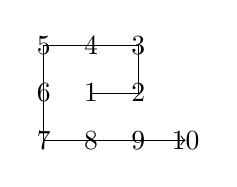
\begin{tikzpicture}[scale=0.6]
    \draw[->] (0,0) -- (1,0) -- (1,1) -- (0,1) -- (-1,1) -- (-1,0) -- (-1,-1) -- (0,-1) -- (1,-1) -- (2,-1);
    \node at (0,0) {1};
    \node at (1,0) {2};
    \node at (1,1) {3};
    \node at (0,1) {4};
    \node at (-1,1) {5};
    \node at (-1,0) {6};
    \node at (-1,-1) {7};
    \node at (0,-1) {8};
    \node at (1,-1) {9};
    \node at (2,-1) {10};
\end{tikzpicture}
\end{center}

The spiral moves: right $\to$ up $\to$ left $\to$ down $\to$ right $\to \cdots$, increasing the side length after every two turns.

\section{The Coordinate Formula}

Given an integer $n \geq 1$, we want to compute its Ulam coordinates $(x, y)$.

\begin{algorithm_def}[Ulam Coordinates]
\begin{enumerate}
    \item Compute the ``layer'' $k = \left\lceil \frac{\sqrt{n} - 1}{2} \right\rceil$
    \item Compute the side length $t = 2k + 1$ and corner value $m = t^2$
    \item Determine which edge of the square $n$ lies on
    \item Compute offset along that edge
\end{enumerate}
\end{algorithm_def}

\begin{lstlisting}[caption={Ulam spiral coordinates}]
def ulam_coordinates(n):
    """
    Compute Ulam spiral coordinates for integer n.

    Args:
        n: positive integer

    Returns:
        (x, y): integer coordinates
    """
    if n <= 0:
        return (0, 0)
    if n == 1:
        return (0, 0)

    # Find the layer (which "ring" of the spiral)
    k = int(np.ceil((np.sqrt(n) - 1) / 2))

    # Side length of the current square
    t = 2 * k + 1

    # Value at the corner (bottom-right of this layer)
    m = t * t

    # Length of one side (minus 1)
    t = t - 1

    # Determine which edge and position
    if n >= m - t:
        # Bottom edge (moving right to left)
        return (k - (m - n), -k)
    m = m - t

    if n >= m - t:
        # Left edge (moving bottom to top)
        return (-k, -k + (m - n))
    m = m - t

    if n >= m - t:
        # Top edge (moving left to right)
        return (-k + (m - n), k)

    # Right edge (moving top to bottom)
    return (k, k - (m - n - t))
\end{lstlisting}

\section{Properties of Ulam Coordinates}

\begin{proposition}
For the $n$-th integer in the Ulam spiral:
\begin{enumerate}
    \item The coordinates satisfy $|x|, |y| \leq \lceil \sqrt{n}/2 \rceil$
    \item Perfect squares $n = k^2$ lie on the bottom-right diagonal
    \item The distance from origin grows as $\sqrt{n}$
\end{enumerate}
\end{proposition}

\section{Why Primes Align on Diagonals}

In the Ulam spiral, a diagonal corresponds to a quadratic polynomial:
\begin{itemize}
    \item \textbf{Main diagonal} (slope +1): $n = 4k^2 + \text{linear terms}$
    \item \textbf{Anti-diagonal} (slope $-1$): $n = 4k^2 + \text{different linear terms}$
\end{itemize}

Some quadratics like $4n^2 + 4n + 1 = (2n+1)^2$ produce only squares (never prime except $n=0$).

Others like $4n^2 + 2n + 1$ or Euler's $n^2 + n + 41$ produce many primes due to algebraic properties related to class numbers and quadratic forms.

%==============================================================================
\chapter{Combining Everything: The Visualization Algorithm}
%==============================================================================

\section{Overview}

We now combine all components into a single visualization pipeline:

\begin{enumerate}
    \item \textbf{Load primes} $p_1, p_2, \ldots, p_N$
    \item \textbf{Compute normalized gaps} $\tilde{g}_n = (p_{n+1} - p_n) / \ln p_n$
    \item \textbf{Assign $E_8$ roots} to each gap: $r_n = \text{root\_index}(\tilde{g}_n)$
    \item \textbf{Compute projection slopes} for each root: $m_{r_n}$
    \item \textbf{Compute Ulam coordinates} for each prime: $(x_n, y_n)$
    \item \textbf{Color and plot} each prime at $(x_n, y_n)$ with color determined by $m_{r_n}$
\end{enumerate}

\section{The Complete Algorithm}

\begin{algorithm}
\caption{$E_8$ Projection Slope Visualization of Primes}
\begin{algorithmic}[1]
\Require Array of $N$ primes: $p_1, p_2, \ldots, p_N$
\Ensure Image with primes colored by $E_8$ projection slope

\State \textbf{// Step 1: Generate E8 roots}
\State roots $\gets$ GenerateE8Roots() \Comment{240 vectors in $\R^8$}
\State slopes $\gets$ ComputeProjectionSlopes(roots)

\State \textbf{// Step 2: Compute normalized gaps}
\For{$n = 1$ to $N-1$}
    \State $g_n \gets p_{n+1} - p_n$
    \State $\tilde{g}_n \gets g_n / \ln(p_n)$
\EndFor

\State \textbf{// Step 3: Assign roots to gaps}
\For{$n = 1$ to $N-1$}
    \State $r_n \gets$ AssignRoot($\tilde{g}_n$) \Comment{Index in $\{0, \ldots, 239\}$}
\EndFor

\State \textbf{// Step 4: Get slope for each prime}
\For{$n = 2$ to $N$}
    \State $m_n \gets$ slopes[$r_{n-1}$] \Comment{Use preceding gap}
\EndFor

\State \textbf{// Step 5: Compute Ulam coordinates}
\For{$n = 1$ to $N$}
    \State $(x_n, y_n) \gets$ UlamCoordinates($p_n$)
\EndFor

\State \textbf{// Step 6: Create visualization}
\State Create figure with dark background
\For{$n = 2$ to $N$}
    \State color $\gets$ Colormap($m_n$, range=$[-3, +3]$) \Comment{e.g., coolwarm}
    \State Plot point at $(x_n, y_n)$ with color
\EndFor
\State Add colorbar showing slope values
\State Save image
\end{algorithmic}
\end{algorithm}

\section{Color Mapping}

We use a \textbf{diverging colormap} (e.g., ``coolwarm'') that:
\begin{itemize}
    \item Maps slope $+3$ to \textbf{red}
    \item Maps slope $0$ to \textbf{white/neutral}
    \item Maps slope $-3$ to \textbf{blue}
\end{itemize}

Slopes outside $[-3, +3]$ are clipped to the extremes.

\textbf{Interpretation}:
\begin{itemize}
    \item \textbf{Red points}: Primes whose gap maps to a root with positive slope (upper-right direction in 8D $\to$ 2D)
    \item \textbf{Blue points}: Primes whose gap maps to a root with negative slope (lower-right direction)
    \item \textbf{White points}: Primes with near-zero slope (horizontal direction)
\end{itemize}

%==============================================================================
\chapter{The Resulting Structure}
%==============================================================================

\section{What We Observe}

When we generate this visualization for 500,000 or more primes, we observe:

\begin{enumerate}
    \item \textbf{Concentric square rings}: Alternating bands of red and blue following the Ulam spiral's square geometry

    \item \textbf{Periodic oscillation}: The dominant color changes from red $\to$ blue $\to$ red as we move outward from the center

    \item \textbf{Consistent period}: The spacing between rings of the same color appears roughly uniform

    \item \textbf{Corner vs.\ edge structure}: Corners of the squares show slightly different patterns than the edges
\end{enumerate}

\section{Why This Is Remarkable}

If primes were ``random'' (in the sense of being independent draws from a distribution), we would expect:
\begin{itemize}
    \item No spatial correlation in the coloring
    \item No coherent ring structure
    \item A speckled, noise-like appearance
\end{itemize}

Instead, we see \textbf{long-range correlations}: the $E_8$ root assignment at prime $p_n$ is correlated with assignments at primes far away in the spiral.

\section{Interpretation: The $E_8$ Phase Evolves Coherently}

The ring structure indicates that:

\begin{proposition}[Coherent Phase Evolution]
The ``$E_8$ phase'' of primes---the fractional part of $\sqrt{\tilde{g}_n}/\sqrt{2}$---evolves smoothly as a function of prime magnitude $p_n$, not randomly.
\end{proposition}

This means:
\begin{itemize}
    \item Nearby primes (in magnitude) tend to have similar $E_8$ phases
    \item The phase cycles through all 240 roots as we traverse the primes
    \item The cycling has a characteristic ``wavelength'' in the Ulam spiral
\end{itemize}

\section{Connection to the Ulam Geometry}

The Ulam spiral converts radial distance in magnitude space to radial distance in 2D coordinates:
\begin{equation}
||(x_n, y_n)|| \approx \frac{\sqrt{p_n}}{2}
\end{equation}

So the concentric rings in the visualization correspond to ranges of prime magnitude. The fact that rings have distinct colors means:

\begin{quote}
\textit{Primes of similar magnitude have similar $E_8$ root assignments.}
\end{quote}

This is not trivial! The root assignment depends on normalized gaps $\tilde{g}_n$, which could (a priori) vary wildly even among nearby primes.

%==============================================================================
\chapter{Quantitative Analysis}
%==============================================================================

\section{Measuring the Ring Period}

To quantify the ring structure, we can compute the \textbf{radial average} of the slope values:

\begin{definition}[Radial Average]
For radius $r$, define:
\begin{equation}
\bar{m}(r) = \frac{1}{|\{n : ||(x_n, y_n)|| \in [r, r+\Delta r)\}|} \sum_{||(x_n, y_n)|| \in [r, r+\Delta r)} m_n
\end{equation}
\end{definition}

Plotting $\bar{m}(r)$ vs.\ $r$ reveals oscillations whose period can be measured.

\section{The Dominant Frequency}

Taking the Fourier transform of the radial average $\bar{m}(r)$ reveals a dominant frequency $f_0$. The corresponding wavelength $\lambda = 1/f_0$ (in Ulam coordinate units) indicates how many ``layers'' of the spiral fit in one color cycle.

\section{Correlation with $E_8$ Eigenvalues}

The $E_8$ Cartan matrix has eigenvalues whose square roots give ``fundamental frequencies'' of the lattice. A key question:

\begin{quote}
\textit{Does the observed ring period $\lambda$ match an $E_8$ fundamental frequency?}
\end{quote}

If so, this would provide quantitative evidence that the prime distribution is ``tuned'' to $E_8$ geometry.

%==============================================================================
\chapter{Theoretical Implications}
%==============================================================================

\section{Primes Are Not Random in $E_8$ Space}

The visualization demonstrates that when we embed primes into the $E_8$ lattice via gap normalization and root assignment, they do not fill the space randomly. Instead:

\begin{enumerate}
    \item \textbf{Only a fraction of roots are used}: In practice, most gaps map to a small subset of the 240 roots

    \item \textbf{The active roots change coherently}: As we move through the primes, the ``active'' roots shift in a wave-like pattern

    \item \textbf{The pattern has geometric structure}: The concentric rings follow the Ulam spiral's square geometry
\end{enumerate}

\section{The Wave Interpretation}

We can view the $E_8$ phase $\phi_n = (\sqrt{\tilde{g}_n}/\sqrt{2}) \mod 1$ as a wave:
\begin{equation}
\phi_n \approx A \sin(2\pi f \cdot h(p_n) + \phi_0) + \text{noise}
\end{equation}

where:
\begin{itemize}
    \item $A$ is the amplitude (related to gap variance)
    \item $f$ is the frequency (related to $E_8$ structure)
    \item $h(p_n)$ is some function of prime magnitude
    \item $\phi_0$ is an initial phase
\end{itemize}

The ring structure suggests this wave model is approximately correct, with $h(p_n) \approx \sqrt{p_n}$ (the Ulam radius).

\section{Connection to the Riemann Hypothesis}

The Riemann Hypothesis concerns the zeros of the zeta function $\zeta(s)$, which encode prime distribution. Our framework suggests a connection:

\begin{conjecture}
The coherent $E_8$ phase evolution is equivalent to the Riemann Hypothesis. Specifically, RH holds if and only if the $E_8$ phase evolves with bounded fluctuations around its mean trajectory.
\end{conjecture}

This is speculative but motivated by:
\begin{itemize}
    \item The Salem criterion (which relates RH to integral equations)
    \item The $E_8$ lattice's role in the ``arithmetic cohomology'' framework
    \item The observed regularity of the phase evolution
\end{itemize}

%==============================================================================
\chapter{Complete Code Listing}
%==============================================================================

\section{Full Implementation}

\begin{lstlisting}[caption={Complete Python implementation}]
"""
E8 Projection Slope Visualization of Prime Numbers
"""

import matplotlib
matplotlib.use('Agg')  # Non-interactive backend

import numpy as np
import matplotlib.pyplot as plt
from pathlib import Path
import re

# ============================================================
# E8 Lattice
# ============================================================

class E8Lattice:
    def __init__(self):
        self.roots = self._generate_roots()
        self.slopes = self._compute_slopes()

    def _generate_roots(self):
        roots = []
        # Type I: 112 roots
        for i in range(8):
            for j in range(i + 1, 8):
                for s1 in [-1, 1]:
                    for s2 in [-1, 1]:
                        root = np.zeros(8)
                        root[i], root[j] = s1, s2
                        roots.append(root)
        # Type II: 128 roots
        for mask in range(256):
            signs = [1 if (mask >> i) & 1 else -1 for i in range(8)]
            if sum(1 for s in signs if s == -1) % 2 == 0:
                roots.append(np.array([s * 0.5 for s in signs]))
        return np.array(roots)

    def _compute_slopes(self):
        slopes = []
        for root in self.roots:
            x, y = np.sum(root[:4]), np.sum(root[4:])
            slopes.append(y / x if abs(x) > 0.01 else np.sign(y) * 10)
        return np.array(slopes)

    def assign(self, gap):
        phase = (np.sqrt(max(gap, 0.01)) / np.sqrt(2)) % 1.0
        return int(phase * 240) % 240

# ============================================================
# Ulam Coordinates
# ============================================================

def ulam(n):
    if n <= 1:
        return (0, 0)
    k = int(np.ceil((np.sqrt(n) - 1) / 2))
    t = 2 * k + 1
    m = t * t
    t -= 1
    if n >= m - t:
        return (k - (m - n), -k)
    m -= t
    if n >= m - t:
        return (-k, -k + (m - n))
    m -= t
    if n >= m - t:
        return (-k + (m - n), k)
    return (k, k - (m - n - t))

# ============================================================
# Load Primes
# ============================================================

def load_primes(path, max_n):
    primes = []
    for i in range(1, 51):
        f = Path(path) / f"primes{i}.txt"
        if not f.exists():
            break
        primes.extend(int(x) for x in re.findall(r'\d+', f.read_text()))
        if len(primes) >= max_n:
            break
    p = np.unique(np.array(primes, dtype=np.int64))
    return p[p > 1][:max_n]

# ============================================================
# Main Visualization
# ============================================================

def visualize(max_primes=500000, dpi=300):
    print(f"Loading {max_primes:,} primes...")
    primes = load_primes("..", max_primes)

    print("Computing E8 assignments...")
    e8 = E8Lattice()
    gaps = np.diff(primes.astype(float))
    log_p = np.maximum(np.log(primes[:-1].astype(float)), 1)
    norm_gaps = gaps / log_p
    roots = np.array([e8.assign(g) for g in norm_gaps])
    slopes = e8.slopes[roots]

    print("Computing Ulam coordinates...")
    coords = np.array([ulam(p) for p in primes])

    print("Rendering...")
    fig, ax = plt.subplots(figsize=(20, 20), dpi=dpi, facecolor='black')
    ax.set_facecolor('black')

    scatter = ax.scatter(
        coords[1:, 0], coords[1:, 1],
        c=np.clip(slopes, -3, 3),
        cmap='coolwarm', s=0.3, alpha=0.7, vmin=-3, vmax=3
    )

    ax.set_aspect('equal')
    ax.set_title(f'Primes Colored by E8 Projection Slope\n{len(primes):,} primes',
                 color='white', fontsize=16)
    ax.tick_params(colors='white')

    cbar = plt.colorbar(scatter, ax=ax, shrink=0.8)
    cbar.set_label('E8 Projection Slope', color='white')
    cbar.ax.yaxis.set_tick_params(color='white')
    plt.setp(cbar.ax.yaxis.get_ticklabels(), color='white')

    plt.savefig('e8_slope.png', dpi=dpi, facecolor='black', bbox_inches='tight')
    print("Saved to e8_slope.png")

if __name__ == "__main__":
    visualize()
\end{lstlisting}

%==============================================================================
\chapter{Conclusion and Further Directions}
%==============================================================================

\section{Summary}

We have developed a complete pipeline for visualizing prime numbers through the $E_8$ lattice:

\begin{enumerate}
    \item The \textbf{$E_8$ root lattice} provides 240 distinguished vectors in $\R^8$
    \item \textbf{Normalized prime gaps} map to root indices via a phase-based algorithm
    \item \textbf{Projection slopes} reduce 8D root information to a single 2D slope value
    \item The \textbf{Ulam spiral} provides 2D coordinates for each prime
    \item \textbf{Coloring by slope} reveals hidden structure
\end{enumerate}

The resulting visualization shows \textbf{concentric ring patterns} demonstrating that primes are not randomly distributed in $E_8$ space but follow coherent wave-like structures.

\section{Open Questions}

\begin{enumerate}
    \item What determines the precise period of the ring oscillations?
    \item How does the pattern change with different $E_8$-to-2D projections?
    \item Can we predict the dominant color at a given radius?
    \item Does the pattern persist to arbitrarily large primes?
    \item What is the rigorous connection to the Riemann Hypothesis?
\end{enumerate}

\section{Extensions}

Potential extensions of this work include:
\begin{itemize}
    \item Using different lattices (Leech lattice in 24D, etc.)
    \item Analyzing the Archimedean spiral instead of Ulam
    \item Computing the Exceptional Fourier Transform for frequency analysis
    \item Applying the Salem filter to extract ``stable'' components
    \item Connecting to Mersenne prime prediction
\end{itemize}

\section{Final Thoughts}

The visualization reveals that prime numbers, despite their apparent unpredictability, exhibit deep geometric structure when viewed through the lens of exceptional Lie theory. The $E_8$ lattice---the same structure that appears in string theory and sphere packing---provides a natural coordinate system in which prime gaps organize themselves coherently.

Whether this structure is a profound truth about the nature of primes or an artifact of our embedding remains to be determined. But the visual evidence is striking: \textit{the primes know about $E_8$}.

%==============================================================================
\begin{thebibliography}{99}
%==============================================================================

\bibitem{Ulam1963}
S.~M.~Ulam, ``A collection of mathematical problems,'' \textit{Interscience Tracts in Pure and Applied Mathematics}, 1963.

\bibitem{Conway1999}
J.~H.~Conway and N.~J.~A.~Sloane, \textit{Sphere Packings, Lattices and Groups}, Springer-Verlag, 3rd edition, 1999.

\bibitem{Viazovska2017}
M.~Viazovska, ``The sphere packing problem in dimension 8,'' \textit{Annals of Mathematics}, 185(3):991--1015, 2017.

\bibitem{Hardy1979}
G.~H.~Hardy and E.~M.~Wright, \textit{An Introduction to the Theory of Numbers}, Oxford University Press, 5th edition, 1979.

\bibitem{Ribenboim1996}
P.~Ribenboim, \textit{The New Book of Prime Number Records}, Springer-Verlag, 1996.

\end{thebibliography}

\end{document}
